For this assignment we will use machine learning techniques to learn a computer 
to play the game Hare and Hounds. Hare and Hounds is a simple game with two players who alternate turns. One player plays as the hare while the other plays as three hounds. The goal of the
hare is to escape the hounds while the goal of the hounds is to capture the
hare. The hare is captured when it cannot move on its turn. The hare has escaped
when it is to the left of at least two hounds, since then it cannot be captured any more.
The board of the game is shown in \autoref{fig:board}. The hounds player is only allowed
to move one hound per turn to adjacent squares that are to the right, either horizontally or
diagonally, or to move vertically. The hare can move in any direction to an adjacent
square. Only one piece is allowed to occupy a square at any time. While this game
seems to be very simple it actually has quite deep strategy.

The game is also known as The Soldier's game, Game of Dwarfs, French Military
Game or any other regional equivalent. Not all of these variants use the same
shaped board but we will focus on the board configuration shown in
\autoref{fig:board}. Other variations include longer or circular boards.
The variant of the game also use different rules. In our variant we have a few
additional rules to those mentioned earlier: the hounds move first and if there 
is no winner after 50 turns, the game is considered a draw.

It is known that when using the rules described above that the game is biased
towards the hounds (SOURCE). Therefore, we expect the hounds to win all games when 
both players are trained. 

In this paper we will describe a method of learning to play the game of Hare
and Hounds using reinforcement learning. The methodology is explained in
\autoref{sec:method}, we discuss the results of training in
\autoref{sec:results} while final remarks are made in \autoref{sec:discussion}.

\begin{figure}[h]
	\centering
	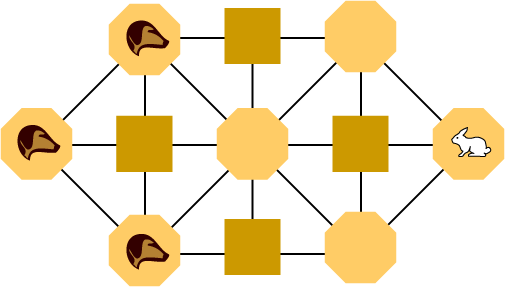
\includegraphics[width=.75\textwidth]{Hare_and_Hounds_board.png}
	\caption{The game board that Hare and Hounds is played on. The hare player
		starts on the right while the hounds player starts on the left.}
	\label{fig:board}
\end{figure}
